% This is samplepaper.tex, a sample chapter demonstrating the
% LLNCS macro package for Springer Computer Science proceedings;
% Version 2.20 of 2017/10/04
%
\documentclass[runningheads]{llncs}
%
\usepackage{graphicx}
%\usepackage{amsthm}
\usepackage{amssymb}
\usepackage{mathtools}
\DeclarePairedDelimiter\abs{\lvert}{\rvert}
\DeclarePairedDelimiter\norm{\lVert}{\rVert}
\DeclarePairedDelimiter\inner{\langle}{\rangle}
\def\P{\mathcal{P}}
\DeclarePairedDelimiter\floor{\lfloor}{\rfloor}
\DeclarePairedDelimiter\ceil{\lceil}{\rceil}

\DeclareMathOperator*{\argmin}{argmin}

\usepackage{algorithm}
\usepackage{algorithmic}
\makeatletter
\newcommand{\algorithmicfunction}{\textbf{function}}
\newcommand{\algorithmicendfunction}{\algorithmicend\ \algorithmicfunction}
\newenvironment{ALC@func}{\begin{ALC@g}}{\end{ALC@g}}
\newcommand{\FUNCTION}[2][default]{\ALC@it\algorithmicfunction\ #2\ %
\textbf{:}%
\ALC@com{#1}\begin{ALC@func}}
\ifthenelse{\boolean{ALC@noend}}{
    \newcommand{\ENDFUNCTION}{\end{ALC@func}}
  }{
    \newcommand{\ENDFUNCTION}{\end{ALC@func}\ALC@it\algorithmicendfunction}
  }
\makeatother

% Used for displaying a sample figure. If possible, figure files should
% be included in EPS format.
%
% If you use the hyperref package, please uncomment the following line
% to display URLs in blue roman font according to Springer's eBook style:
% \renewcommand\UrlFont{\color{blue}\rmfamily}

\begin{document}
%
\title{Info-Detection: An Information-Theoretic Approach to Detect Outlier}
%
%\titlerunning{Abbreviated paper title}
% If the paper title is too long for the running head, you can set
% an abbreviated paper title here
%
\author{Feng Zhao\inst{1} \and
Fei Ma\inst{2} \and
Yang Li\inst{2} \and
Shao-Lun Huang \inst{2} \and
Lin Zhang\inst{1,2}}
%
\authorrunning{Feng Zhao et al.}
% First names are abbreviated in the running head.
% If there are more than two authors, 'et al.' is used.
%
\institute{Department of Electronic Engineering, Tsinghua University \and
Tsinghua-Berkeley Shenzhen Institute, Tsinghua University \\
\email{zhaof17@mails.tsinghua.edu.cn}
}
%
\maketitle              % typeset the header of the contribution
%
\begin{abstract}
Outlier detection is one of major task in unsupervised learning. We propose a cluster analysis based outlier detection method called Info-Detection. Info-Detection determines the number of outliers automatically and captures the global property of the provided data. To implement Info-Detection and overcome the global computational complexity, we use principal sequence of partition, which we improve one order of magnitude faster than the original version. Experiments show that compared with other outlier detection methods, Info-Detection achieves better accuracy with an affordable time overhead.

\keywords{Outlier Detection \and Clustering \and Principal Sequence of Partition.}
\end{abstract}
%
%
%
\section{Introduction}
Outlier detection is an important task in data mining. It is the identification of abnormal data (called outliers) which differ from the majority of the data (called inliers) \cite{grubbs1969procedures}. It has applications in fraud detection, loan application processing, activity monitoring etc.\cite{Hodge2004}. Many existing detection algorithms give an outlier score to each data point and the outliers are chosen as those points with highest scores. These methods need to know the number of outliers $n$ in advance but for real-world task, we do not know how many outliers there are and mismatched $n$ produces no good result. Also, besides distance metric, many outlier detection methods have other hyper parameters to tune, which depends heavily on dataset. 

To overcome these problems, we propose Info-Detection, which do not require $n$ in advance and is determined totally by the similarity metric used.  
Info-Detection is a cluster analysis based method. Some authors use density-based cluster method to do outlier detection \cite{Campello}. But density method only captures the local property of the data. When outliers are concentrated, density-based method fails to report the truth. Info-Detection comes from info-clustering, which is a global clustering method \cite{RN1} and does not have this problem. Info-clustering has solid theoretical foundations from information theory and can produce hierarchical tree for the random variables to be clustered. Info-clustering can also be used to cluster data. In such case, it produces the same clustering result as minimum cost clustering with $\beta = 1$ in \cite{RN7}. In this paper, we combine info-clustering with graph theory and propose Info-Detection, which captures the global property of the dataset.  

Though info-clustering has good theoretical properties, it has high time complexity to compute, which limited its application. In this paper, we improve the implementation of info-clustering, which is one order of magnitude faster than the original one. We also propose a prediction scheme which can predict new observations in linear time complexity. To demonstrate our method works, we prepare two artificial and two real-world dataset and test Info-Detection and other methods on them. Empirical comparison shows that Info-Detection gives best result on these datasets and is suitable for different kinds of data.

The paper is organized as follows. In Section \ref{sec:ID}, we make a brief introduction of info-clustering and propose Info-Detection. In Section \ref{sec:Alg}, we review the original algorithm of info-clustering and give our new accelerated implementation. In Section \ref{sec:Experiemt}, we conduct experiments of outlier detection and compare Info-Detection with other methods. Finally, we make the conclusion in Section \ref{sec:Conclusion}. Proposition proof and other supplementary materials are provided in the Appendix.

The notation convention of this paper is as follows: Let $x_i$ represents the feature vector for the $i$-th data point in the dataset. The directed graph is denoted by $G(V, E)$. Node index set $V=\{1, 2,\dots, \abs{V}\}$. Node set $Z_V=\{Z_i | i \in V\}$. Edge set $E$ is the collection of tuple $(i,j)$. For $B\subseteq V$, edge subset $E(B) = \{(i,j)| i, j \in B,(i,j)\in E\}$ is the edge set restricted on $B$. Each edge is associated with a non-negative weight $w_{ij}$, which is computed from $x_i$ and $x_j$ with a given affinity metric. $\P$ is a partition of $V$. That is, $P=\{C_1, \dots, C_k\}, \cup_{i=1}^k C_i=V$ and $i\neq j \Rightarrow C_i \cap C_j =\emptyset $. $F(\cdot)$ is the graph in-cut function, defined as $f(C)=\sum_{i \neq C, j\in C, (i,j) \in E} w_{ij}$. $\Pi$ is the collection of all partitions of $V$ and $\Pi'=\Pi\backslash\{V\}$. A partial order $ \P_1 \preceq \P_2$ on $\Pi$ is defined as
$C \in \P_1 \Rightarrow \exists C' \in \P_2 \, s.t. \, C \subseteq C'$.
Finally, $f[\cdot]$ is a function defined on $\Pi$ by $f[\P]=\sum_{C\in \P}f(C)$ and $\textrm{maximal} (F)=\{B\in F | \not\exists B' \in F s.t.\, B \subseteq B'\}$.

\section{Formulation of Info-Detection}\label{sec:ID}
\subsection{Overview of Info-clustering}
Info-Detection comes from info-clustering \cite{RN1}. For a graph $G(V,E)$, info-clustering defines the cluster as follows:
\begin{align}
I_{\P}(Z_V) & := \frac{ f[\P] }{  \abs{\mathcal{P}} - 1 }\\
I(Z_V) & := \min_{\mathcal{P} \in \Pi'(V)} I_{\mathcal{P}}(Z_V)  \label{eq:ms} \\
C_{\gamma}(Z_V) & := \textrm{maximal}\{ B \in V \vert \, \abs{B} > 1, I(Z_B) > \gamma \} \label{eq:CgZv}
\end{align}
where $I(Z_B)$ is the shared information of $Z_B$. For the definition of $I_{\P}(Z_B)$, the subgraph $G(B,E(B))$ is considered instead.

For the given threshold $\gamma$, $C_{\gamma} (Z_V)$ represents a collection of non-intersecting subset of $V$. Every two sets from $\bigcup_{\gamma \geq 0} C_{\gamma}(Z_V)$ are either disjoint or have subset relationship. Therefore, they can be put in a tree $\mathcal{T}$ with the property that $A$ is a parent of $B$ if $B\subset A$. $\mathcal{T}$ also includes $\{j\}$ as leaf node. 

For sufficiently large $\gamma$, $C_{\gamma} (Z_V)$ will become empty set. The largest threshold value which makes such transition is denoted by $\gamma_N$, which has the following expression:
\begin{equation}\label{eq:gammaN}
\gamma_N = \max_{A\subseteq V, \abs{A}>1} I(Z_A)
\end{equation}
Suppose $\gamma_N=I(Z_B)$ and $B$ is maximal in a sense of equation \eqref{eq:CgZv}. This convention is used in the following paper.
It is shown in \cite{RN8} that $\gamma_N$ has an alternative form
\begin{equation}\label{eq:gammaN_alternative}
\gamma_N = \max_{A \subseteq V, \abs{A}>1} \frac{\sum_{(i,j)\in E(A)} w_{ij}}{\abs{A}-1}
\end{equation}
In agglomerative interpretation of info-clustering \cite{RN8}, each singleton element $\{i\}$ is regarded as a leaf node of the hierarchical tree. $\gamma_N$ represents the first step to process the leaf node. That is, merging elements of $B$ to form a stem node. Traditional hierarchical clustering method using linkage criterion restricts $\abs{A}=2$ in the maximization of equation \eqref{eq:gammaN_alternative}. The information criterion $\gamma_N$ does not have such restriction. 
\subsection{Info-Detection Method}
For our Info-Detection proposal, we use $\gamma_N$ as a threshold to detect anomaly. Given $G(V, E)$, we first compute $\gamma_N$ and $B$. Then nodes in $B$ are inliers while nodes in $V\backslash B$  are outliers. We can score outlier $Z_j$ for $j \in V\backslash B$ with the depth of the set $\{j\}$ in the hierarchical tree. Below is a simple example showing how Info-Detection is used.
\begin{example}
	\begin{figure}[!ht]
		\centering
		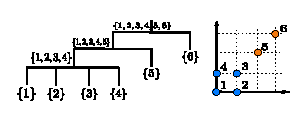
\includegraphics[width=9cm]{pic/outlier_example.eps}
		\caption{Info-Detection applied to 6 points on Cartesian plane}\label{fig:ex}
	\end{figure}
	Consider a graph consisting of 6 nodes. Each node is corresponding to a point on Cartesian plane (Fig. \ref{fig:ex}.(b)). The grid has one unit and the edge weight $w_{ij} = \exp(-d_{ij}^2)$ where $d_{ij}$ is the Euclidean distance of $x_i$ and $x_j$ on the plane. For example, $w_{45} = \exp(-5)$. The edge direction is from $i$ to $j$ for $i<j$. From equation \eqref{eq:gammaN}, we can compute $B=\{1,2,3,4\}$ and $\gamma_N = \frac{4\exp(-1)+2\exp(-2)}{3}\approx 0.58$. The whole hierarchical tree $\mathcal{T}$ can also be computed, which is shown on Fig. \ref{fig:ex}.(a). The outlier score for $Z_6$ is higher than $Z_5$ from the tree depth interpretation.
\end{example}
For newly added node $i'$. Let $V'=B\cup \{i'\}$, we can compute $\gamma'_N$ for $G(V', E(V'))$ and compare it with $\gamma_N$. If $\gamma'_N>\gamma_N$, $i'$ is normal observation since it is more integrated with existing nodes. Otherwise, $i'$ is anomaly. It can be shown that we do not need to compute $\gamma'_N$ to determine whether $\gamma'_N>\gamma_N$. We summarize our main result as follows:
\begin{proposition}\label{prop:main}
\begin{equation}
\gamma'_N > \gamma_N \iff  \sum_{i \in B} w_{ii'} > \gamma_N 
\end{equation}
\end{proposition}
From Proposition \ref{prop:main}, we can see that the computational overhead to check whether new data is normal is linear to the size of existing normal data. 

Info-Detection requires $\gamma_N$ and $B$, whose computation is not a trivial task, whose computation is the main focus of the next Section.

\section{Improved Principal Sequence of Partition}\label{sec:Alg}
\subsection{Existing Algorithms}
It has been found that the mathematical structure of info-clustering is the same with that of principal sequence of partition (PSP) of graph. We use $\P_1, \dots, \P_k$ to denote PSP sequence where $\P_1 = \{V\}, \P_{i+1} \preceq \P_i$ and $\P_k = \{\{1\},\dots,\{k\}\}$.
Each $\P_i$ is the solution to the following optimization problem:
\begin{align}
h_{\P}(\lambda) &=  f[\P] - \abs{\P} \lambda  \label{eq:hPL}\\
h(\lambda) &= \min_{\P \in \Pi'(V)} h_{\P}(\lambda) \label{eq:hlambda}
\end{align}
We call $\lambda^*$ is a critical value for PSP if $\P_i, \P_{i+1}$ are both minimizer for $h(\lambda^*)$ in \eqref{eq:hlambda}.
The largest critical value is equal to $\gamma_N$ and the largest set in $\P_{k-1}$ is equal to $B$. 

Info-clustering is originally implemented by solving equation \eqref{eq:hlambda} for different critical values \cite{RN3}. For given critical value, a procedure called Dilworth truncation (DT) can be used to get the minimum value and corresponding partition. This implementation has $\abs{V}^2 \textrm{MF}(G)$ time complexity while \textrm{MF} represents the time complexity of maximum flow algorithm for a graph $G$. 

An improvement is proposed in \cite{RN4} using parametric maximum flow to finish the job. Although this method can achieve $\abs{V} \textrm{MF}(G)$ theoretically, it also increases the spacial complexity to $ \abs{V} \textrm{S}(G)$ where $\textrm{S}$ represents the spacial complexity to store a graph structure $G$. For dense graphs with $\abs{V}^2$ non-zero floating-point weight, the spacial complexity $\abs{V}^3$ is formidable. 
% analysis of spatial complexity of pmf
Another problem of parametric maximum flow implementation is the floating point accuracy. Since this method uses the flow map of last computation to initiate the initial flow map of next computation for maximal flow algorithm, the excess flow of some nodes may not be exactly zero. The non-zero excess can lead to unpredictable result and currently there is no good idea to tackle this issue. The above two problems prohibits parametric implementation from practical usage.

In this section, we give an improvement which achieves $\abs{V} \textrm{MF}(G)$ time complexity in general, but with only $\textrm{S}(G)$ spatial complexity and no floating point issue. Specifically,
we notice that different invocation of Dilworth truncation is independent and does not utilize the intrinsic hierarchical structure in the original version of PSP algorithm \cite{RN3}. By using the hierarchical tree structure, we can invoke Dilworth truncation on smaller graph in later computation and make the total computation one order of magnitude faster than previous.

\subsection{Improved Algorithm} 
Since the PSP has the inclusion relationship $\P_{i+1} \preceq \P_i$, we can restrict further invocation of DT to smaller graphs. To be more specific, suppose we get $P_i = {C_1, \dots, C_t}$ for the first invocation of DT. Then we can compute PSP for each $C_i(i=1,\dots, t)$ respectively and construct those $P_j(j>i)$ from the subgraph computation. For $P_j(j<i)$, we can contract the graph $G$  to $G^t$ which has $t$ nodes by contracting each $C_i$ to a single node. By applying DT to $G^t$ can we get $P_j(j<i)$. We summarize our improved version in Algorithm \ref{alg:psp_i_simplified}.

\begin{algorithm}
	\caption{An Improved Principal Sequence of Partition Algorithm}\label{alg:psp_i_simplified}
	\begin{algorithmic}[1]
		\REQUIRE a directed graph $G(V, E)$; edge weight map $c(e)$ for $e\in E$
		\ENSURE a hierarchical tree $\mathcal{T}(K, E)$ where $K \subseteq 2^{V}$ is node set and $E$ is edge set. $c'$ is edge weight map.
		\STATE initialize tree $\mathcal{T}$ with $V$ as root node, $\{j\}(j\leq \abs{V})$ as leaf node and no stem node.
		\STATE \texttt{Split}($G, V$)
		\FUNCTION{\texttt{Split}($\widetilde{G}, \widetilde{V}$)}
		\STATE $w$ is the summation of all edge weights of $\widetilde{G}$ 
		\STATE $\gamma' = \frac{w}{\abs{V(\widetilde{G})}-1}$ where $V(\widetilde{G})$ is the node set of graph $\widetilde{G}$ \label{alg:gamma_apostrophe}
		\STATE $(\tilde{h}, P') = \texttt{DT}(\widetilde{G}, \gamma')$ where $\P'$ is minimizer of equation \eqref{eq:hlambda} and $\tilde{h}$ is the corresponding minimum value.  \label{alg:DT}
		\IF{$\tilde{h} = - \gamma'$}
		\STATE add edge weight $\gamma'$ in $\mathcal{T}$ starting from $\widetilde{V}$ to its children.
		\ELSE
		\FOR{$S$ in $P'$ and $\abs{S}>1$}
		\STATE make each children of $\widetilde{V}$ in $\mathcal{T}$ have new parent $S$		
		\STATE make the parent of $S$ be $\widetilde{V}$
		\STATE \texttt{Split}($\widetilde{G}[S], S$) where $\widetilde{G}[S]$ is the subgraph of $\widetilde{G}$ restricted on $S$
		\STATE contract $S$ to a single node in $\widetilde{G}$ % graph \widetilde{G} is modified
		\ENDFOR 
		\STATE \texttt{Split}($\widetilde{G}, \widetilde{V}$)		
		\ENDIF
		\ENDFUNCTION
	\end{algorithmic}
\end{algorithm}
	
\begin{figure}[!ht]
	\centering
	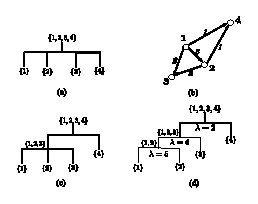
\includegraphics[width=9cm]{pic/alg_illustration.eps}
	\caption{Improved PSP for the graph in (b), hierarchical tree evolves from (a), (c) to (d) }\label{fig:alg_eg}
\end{figure}

\begin{example}
	We use a simple example to explain Algorithm \ref{alg:psp_i_simplified}. Consider a graph $G(V, E)$ with $V=\{1,2,3,4\}, E=\{(1,2),(1,3),(2,3),(1,4),(2,4)\}$. The weight values are $w_{13}=2, w_{12}=5, w_{23}=2, w_{14}=1, w_{24}=1$. The graph is illustrated
	in Fig. \ref{fig:alg_eg} (b). Initially, the hierarchical tree is shown in Fig. \ref{fig:alg_eg} (a). Computing $\gamma' = \frac{11}{4-1}, \tilde{h} = -\frac{16}{3} < -\gamma' $ and $\P' = \{\{1,2,3\},\{4\}\}$ from line \ref {alg:DT} in Algorithm \ref{alg:psp_i_simplified} we get the hierarchical tree shown in Fig. \ref{fig:alg_eg} (c).
	
	Then we run PSP for the subgraph $G[\{1,2,3\}]$, $\gamma' = \frac{9}{2}, \tilde{h} = -5 < -\gamma'$ and $\P= \{\{1,2\},\{3\}\}$ we get the tree shown in Fig. \ref{fig:alg_eg} (d). The other computation calculate the edge weight of $\mathcal{T}$ shown in Fig. \ref{fig:alg_eg} (d).
\end{example}		

To analyze the time complexity of Algorithm \ref{alg:psp_i_simplified}. We suppose $\abs{V} = n, \abs{E} = O(n^2)$ and highest-relabel preflow algorithm is used to solve the maximum flow problem. Then \texttt{DT} routine has $O(n^4)$ time complexity. 
We use $T(n)$ to represent the time complexity of \texttt{Split} when the graph has $n$ nodes. Under very general conditions, we can show that $T(n) = O(n^4)$. The detailed analysis is put in the Appendix \ref{sec:AA}.

In Algorithm \ref{alg:psp_i_simplified}, the computation is done on the input graph and only has $O(n^2)$ space complexity. This is superior than parametric preflow improvement. Besides, Algorithm \ref{alg:psp_i_simplified} does not have floating accuracy problem since each DT computation is freshly started. 

Our improvement of algorithm is not restricted to Info-Detection scenario. It can be used in general graph partition problems when PSP structure is needed.

\section{Experiment Result}\label{sec:Experiemt}
In this Section, we first illustrate the decision boundary of Info-Detection by two artificial datasets. Then we conduct an experiment matrix, in which Info-Detection is compared with other commonly used outlier detection algorithms on both artificial and real-world datasets.

The first artificial dataset is two Gaussian blobs with the same center and standard deviation 0.5. There are 255 points in total and 45 noisy points outside.
The second dataset is two semi-circles which located at different centers. There are 300 points on the two semi-circles, which are evenly distributed among the angle but deviated from the radius in Gaussian distribution. There are 45 points not belonging to the "moon" structure and are treated as outlier.

Info-Detection first splits each dataset into inlier set and outlier set. Then the boundary curve is generated from the inlier set. The curve has the following equation from Proposition \ref{prop:main}:
\begin{equation}
\sum_{j \in B} \exp(-\gamma \norm{x - x_j}^2)= \gamma_N
\end{equation}
The weight is chosen by Gaussian kernel, which produces reasonable good result for these two artificial dataset. As shown by Fig. \ref{fig:boundary}.(a) and (b), the boundary curve for Info-Detection is approximately the closure of the set of inliers. We also draw the decision boundary for the elliptic envelope method in Fig. \ref{fig:boundary}.(c). Since the latter method assumes the inlier data is distributed in convex region, the decision boundary is an ellipse, which is not the ground truth and inferior to figure of Info-Detection.
\begin{figure}[!ht]
	\centering
	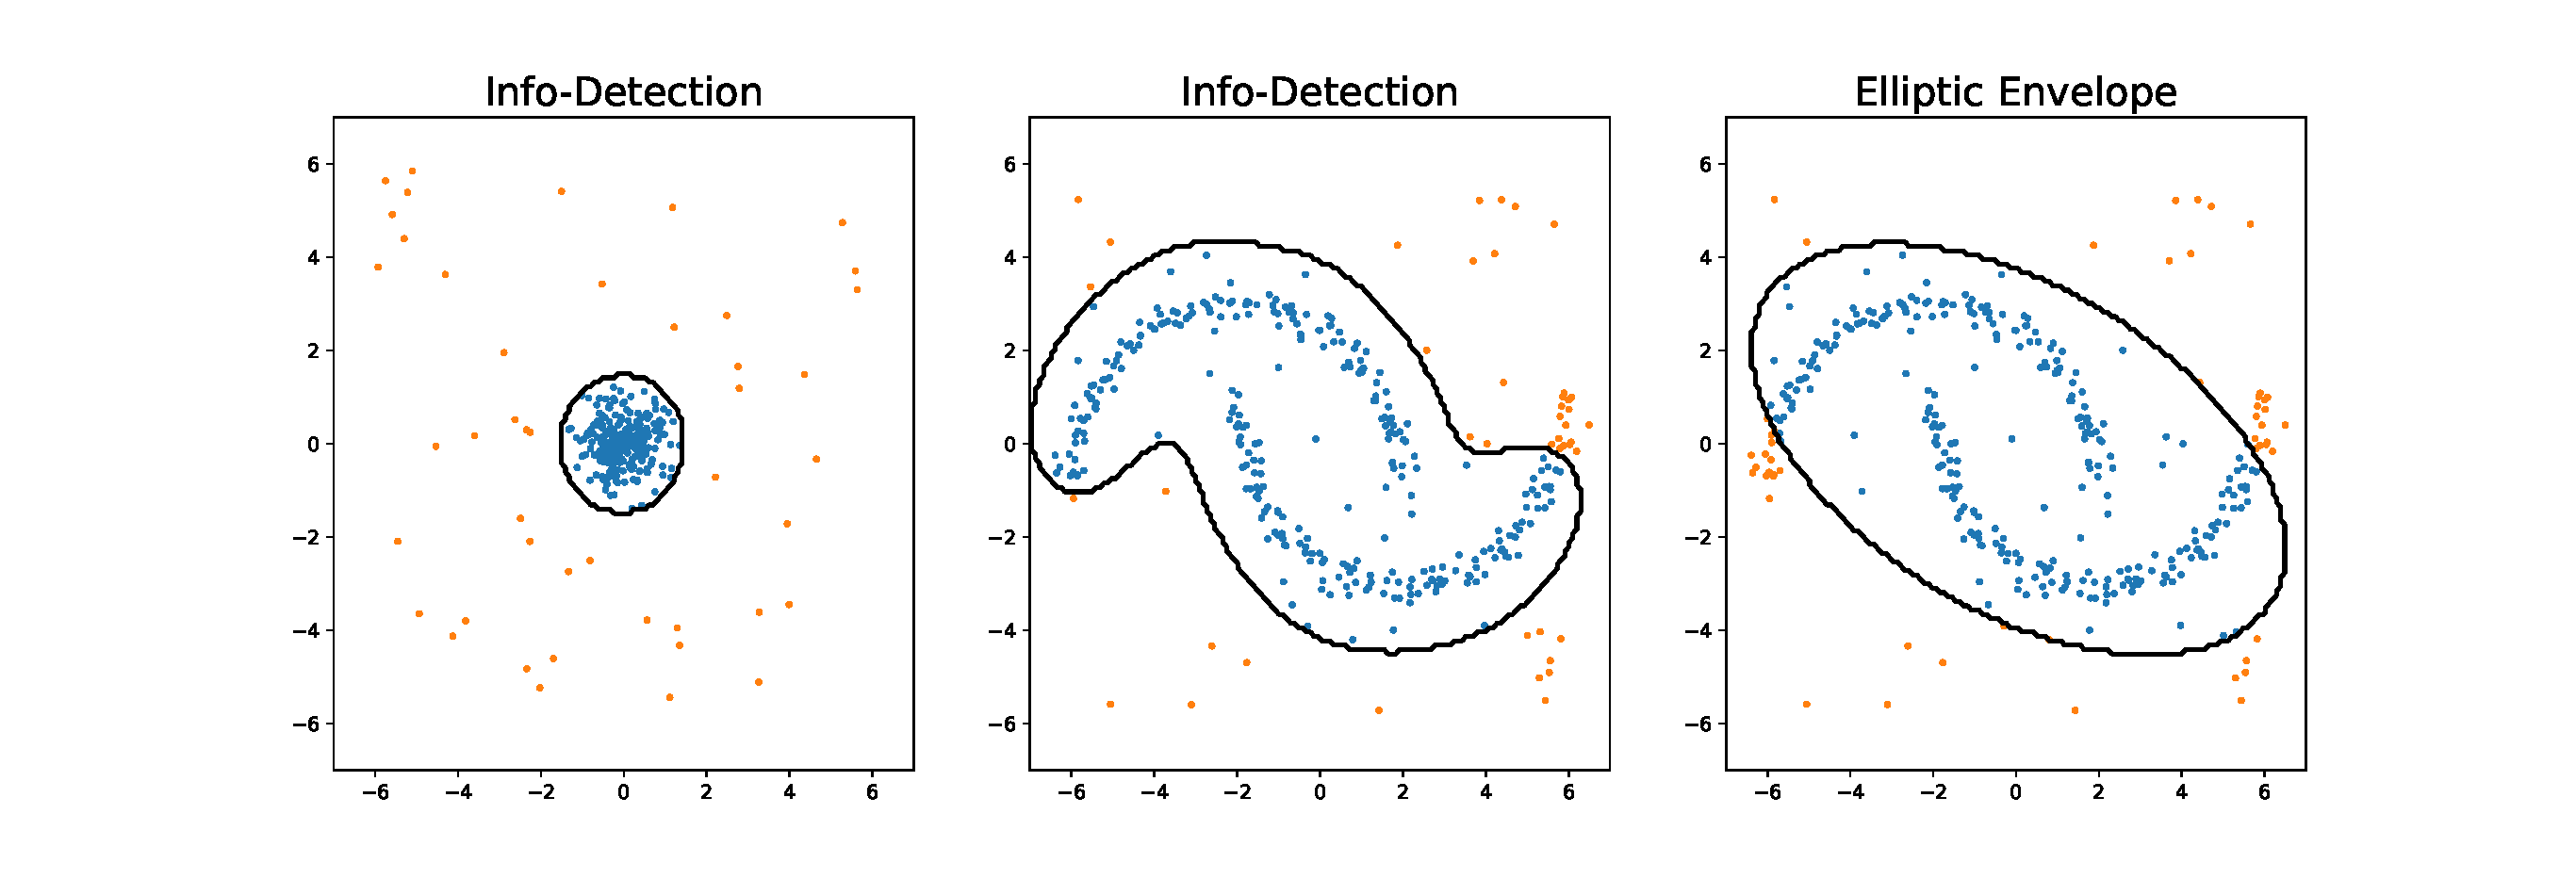
\includegraphics[width=\textwidth]{pic/outlier_boundary_illustration.eps}
	\caption{Detection boundary lines of different methods on different artificial dataset}	\label{fig:boundary}
\end{figure}

Besides the two artificial dataset, we also prepare two real-world datasets: Lymphography (first used by \cite{Lazarevic}) and Glass (\cite{hics}). Lymphography dataset has 148 instances with 19 attributes and 6 outliers while Glass dataset has 214 instances with 7 attributes and 7 outliers. We compare Info-Detection method with four commonly used techniques: local outlier factor \cite{Breunig}, isolation forest \cite{if}, elliptic envelope \cite{rousseeuw1999fast} and one class SVM \cite{svm}. We use two metrics to measure the overall performance of the detection: true positive rate (TPR) and false negative rate (FNR). The inlier is treated as positive sample. TPR measures the percentage of right detection in inlier set while FNR measures that in outlier set. It is difficult for a method to achieve high score on both two metrics. We manage to maximize FNR while controlling TPR $\geq 90\%$. The result is shown in Table \ref{tab:compare}.
\begin{table}[!ht]
\centering
\InputIfFileExists{../../experiment/outlier_detection/build/id_compare.tex}{}{}
\caption{Comparison of Info-Detection with other outlier detection algorithms on artificial and real-world datasets}\label{tab:compare}
\end{table}

All results in Table \ref{tab:compare} achieves TPR $\geq 90\%$. It can be seen that Info-Detection achieves highest FNR for these datasets, which means Info-Detection detects no less outliers than other methods.

\section{Conclusion}\label{sec:Conclusion}
In this paper, we propose Info-Detection, which is a cluster analysis based method and does not require the number of outliers in advance. We design an efficient algorithm to get the hierarchical structure of data based on existing PSP algorithms. By experiments we show that Info-Detection outperforms other methods.  
%
% ---- Bibliography ----
%
% BibTeX users should specify bibliography style 'splncs04'.
% References will then be sorted and formatted in the correct style.
%
\bibliographystyle{splncs04}
\bibliography{exportlist}
%
\appendix
\section{Proposition Proofs}
\begin{proof}[Proof of Proposition \ref{prop:main}]
		In this proof, we make some notation convention.
		$w(C) = \displaystyle\sum_{(i,j) \in E(C)} w_{ij},$
		$w(A, C) = \displaystyle\sum_{\substack{i \in A, j \in C \\ (i,j) \in E(V')}} (w_{ij}+w_{ji})$ and
		$\P_C = \{\{i \}| i \in C \}$. Suppose $\gamma_N = I(Z_B)$, from equation \eqref{eq:gammaN}, we can get $\gamma_N =\frac{f[\P_B]} {\abs{B} -1}$.
		Since $V' = B \cup \{i'\}$
		$f[\P_{V'}] = f[\P_B] + \sum_{i \in B}w_{ii'}$.
		
		If $ \sum_{i \in B} w_{ij} > \gamma_N$ we can get
		$$
		\gamma'_N \geq I_{\P_{V'}}(Z_{V'}) = \frac{(\abs{B}-1)\gamma_N + \sum_{i \in B}w_{ii'}}{\abs{B}} > \gamma_N
		$$
		
		On the other hand, suppose $\gamma'_N = I(Z_K) > \gamma_N$. Then $K$ must contain $i'$. If $K=V'$ then the conclusion holds. Otherwise, Suppose $K = \{i'\} \cup B', B=B'\cup J, J\neq \emptyset$. We can write 
		\begin{equation}\label{eq:gammaNF}
		\gamma_N = \frac{w(J,B') + w(J) + w(B')}{ \abs{B'} + \abs{J} - 1 }
		\end{equation}
		Since $I(Z_K) = I_{\P_K}(Z_K)$ is maximal, we have $I_{\P_K}(Z_K) > I_{\P_{V'}}(Z_{V'})$ and $I_{\P_K}(Z_K) \geq I_{\P_{B'}}(Z_{B'})$.
		\begin{align*}
			\frac{w(\{i'\}, B') + w(B')}{\abs{B'}} >& \frac{w(B') + w(J, B') + w(J) + w(\{i'\}, B') + w(\{i'\}, J)}{\abs{B'} + \abs{J}}  \\
			\frac{w(\{i'\}, B') + w(B')}{\abs{B'}} \geq & \frac{w(B')}{\abs{B'} - 1}
		\end{align*}
		we can get 
		\begin{align}
			\abs{J} (w(\{i'\}, B') + w(B')) > & \abs{B'} (w(J, B') + w(J) + w(\{i'\}, J)) \label{eq:target}
			\\
			(\abs{B'} - 1)  w(\{i'\}, B') \geq & w(B') \label{eq:convert}
		\end{align}
		Take equation \eqref{eq:convert} in \eqref{eq:target}, we can get
		\begin{equation}\label{eq:summation}
		\abs{J} w(\{i'\}, B') > w(J, B') + w(J) + w(\{i'\}, J)
		\end{equation}	
		Combined with \eqref{eq:gammaNF}, adding equation \eqref{eq:convert} and \eqref{eq:summation} we can get
		$w(\{i'\}, B') > \gamma_N$. Then $\sum_{j \in B}w_{ii'} > \gamma_N $ follows.
\end{proof}	
\section{Algorithm Analysis}\label{sec:AA}
In this section, we give detailed analysis of time complexity of Algorithm \ref{alg:psp_i_simplified}.
It is noticed that each invocation of \texttt{Split} makes the graph $\widetilde{G}$ contract at least two nodes. Therefore, at most $\abs{V}-2$ times \texttt{Split} is called. Suppose the time complexity of \texttt{DT} is bounded by $Cn^4$. Then in worst scenario, the complexity bound for \texttt{Split} is $C(3^4+4^4 + \dots + n^4) \sim \frac{1}{5}Cn^5$, which is $5$ times faster than the original PSP algorithm $Cn^5$.

Generally, this worst case is not reached. The recursive relationship for $T(n)$ is
\begin{equation}\label{eq:Tn}
T(n) = \max \{ C n^4 + \sum_{i=1}^k T(n_i) + T(k) | \sum_{i=1}^k n_i = n, n_i \in \mathbb{Z}_{+} \}
\end{equation}	
For graph $\widetilde{G}$, let $\lambda_1(\widetilde{G}) < \dots < \lambda_k(\widetilde{G})$ be its critical value list. $\gamma'(\widetilde{G})$ comes from line \ref{alg:gamma_apostrophe} in Algorithm \ref{alg:psp_i_simplified} and $\floor{x}, \ceil{x}$ represent floor, ceil respectively.
We have the following proposition:
\begin{proposition}\label{prop:alg_complexity}
	If $\abs{E} = O(n^2)$ and $ \lambda_{\floor{k/2} - 1}(\widetilde{G}) \leq \gamma'(\widetilde{G}) \leq \lambda_{\ceil{k/2} + 1}(\widetilde{G}) $ holds for each invocation of function \texttt{Split}, then $T(n) = O(n^4)$.
\end{proposition}
\begin{proof}
	$\lambda_{\floor{k/2} - 1} \leq \gamma' \Rightarrow n_i \leq \frac{n}{2}$ and $ \gamma' \leq \lambda_{\ceil{k/2} + 1} \Rightarrow k < \frac{n}{2} $ in equation \eqref{eq:Tn}. Let $\mu_i = \frac{n_i}{n}$. We proceed by induction to show $T(n) = O(n^4)$. More specifically, $T(n) \leq q C n^4$ where $ q = \frac{16}{5}$. $T(3)$ is a constant and $T(m) \leq q C m^4$ holds for $m=3$. Suppose
	$T(m) \leq qC m^4$ holds for all $m \leq n-1$. Then for $T(n)$
	We first show that 
	\begin{equation}\label{eq:outerI}
	\sum_{i=1}^k T(n_i) \leq 10 T(\frac{n}{2})
	\end{equation}
	Since $\sum_{i=1}^k T(n_i) \leq qC n^4\sum_{i=1}^k u_i^4$ and $10 T(\frac{n}{2}) \geq 10Cn^4 (\frac{1}{2})^4$ from equation \eqref{eq:Tn}
	\begin{equation}\label{eq:innerI}
       q\sum_{i=1}^k u_i^4 \leq 10 (\frac{1}{2})^4 
	\end{equation}
	We have \eqref{eq:innerI} $\Rightarrow$ \eqref{eq:outerI}. The constraint is that $u_1\leq u_2 \leq \dots \leq u_k \leq \frac{1}{2}$ and $\sum_{i=1}^k u_i = 1$. Therefore we have $u_1 \leq \frac{1}{k}, u_2 \leq \frac{1}{k-1}, \dots, u_{k-1} \leq \frac{1}{2}$.
	\begin{equation}\label{eq:outerOne}
	 q[2(\frac{1}{2})^4 + \sum_{i=3}^k (\frac{1}{i})^4] \leq 10 (\frac{1}{2})^4
	\end{equation}
	We have \eqref{eq:outerOne} $\Rightarrow$ \eqref{eq:innerI}. And \eqref{eq:outerOne} is equivalent to
	$\sum_{i=3}^k (\frac{1}{i})^4 \leq \frac{9}{8}(\frac{1}{2})^4$
	\begin{align*}
		\sum_{i=3}^k (\frac{1}{i})^4 & < \frac{1}{9}\sum_{i=3}^k (\frac{1}{i})^2 \\
		& < \frac{1}{9}\sum_{i=3}^k (\frac{1}{(i-1)i}) \\
		& < \frac{1}{18} < \frac{9}{8}(\frac{1}{2})^4
	\end{align*}
	Therefore, \eqref{eq:outerI} holds and from \eqref{eq:Tn} we have 
	\begin{align}
		T(n)  & \leq Cn^4 + 11T(\frac{n}{2}) \\
		& \leq C n^4 + 11 q C (\frac{n}{2})^4 = \frac{16}{5} C n^4
	\end{align}
\end{proof}	
\begin{remark}
		Using the agglomerative view of info-clustering, we can show that 	$\gamma'$ is weighted average of $\lambda_1, \dots, \lambda_k$. Indeed, we can
		get a successively increasing set $\emptyset = S_0 \subsetneq S_1 \subsetneq S_2 \subsetneq \dots \subsetneq S_k$ such that $S_k = V$. Let $\delta_{11}=1, \delta_{i1}=0$ for $i\neq 1, \gamma_i = \frac{\sum_{(i,j) \in E(S_i\backslash S_{i-1})} w_{ij}}{\abs{S_i\backslash S_{i-1}}- \delta_{i1}}$. Then we have $\gamma' = \sum_{i=1}^k \frac{\abs{S_i \backslash S_{i-1}} - \delta_{i1}}{\abs{V} - 1}\gamma_i$ from the definition of $\gamma'$. The agglomerative interpretation contracts the graph from $S_1$ to $S_k$ and each contraction computes a critical value $\lambda_i = \gamma_{k-i+1}$.
		
		The condition added by Proposition \ref{prop:alg_complexity} says if the weighted average of $\lambda_i$ is near to its median, then $T(n) = O(n^4)$. We believe this result can be obtained under a more tolerant condition.
\end{remark}		
\section{Experiment Detail}
Since Info-Detection is a graph-based method, how to choose graph weight $w_{ij} = \mathrm{affinity}(x_i, x_j)$ is important for practical application of Info-Detection. For our experiment, we use Gaussian kernel $w_{ij} = \exp(-\gamma \norm{x_i - x_j}^2)$, Laplacian kernel $w_{ij} = \exp(-\gamma \norm{x_i - x_j}_1)$. We also try k-neighbor filtering. That is, after comting $w_{ij}$, we only preserve the largest $k$ weight. Suppose $w_{i1} > w_{i2} > \dots > w_{in}$, then
$$
w'_{ij}  = 
\begin{cases}
 w_{ij} & j \leq k \\
 0 & j > k
\end{cases}
$$
By using $k$-neighbor filtering, the graph has less edge and Info-Detection can run much faster. On the other hand, it restricts the linkage of graph node to its k-nearest neighbors, which makes Info-Detection more robust.

The source code of our experiment is available \footnote{\scriptsize\url{https://github.com/zhaofeng-shu33/info-detection-experiment}} for reproduction.
For our experiment comparison, the accuracy of isolation-forest and elliptic envelope is influenced by their intrinsic randomness. With the same parameter configuration, we select the result of one run of it, not possibly the best result. Info-Detection, one class SVM and local outlier detector are deterministic method and do not have this problem.
For local outlier factor, isolation forest and elliptic envelope, they need to know the number of outliers in advance. We set this parameter to be ground truth for these three methods to produce best result. We also tune the number of neighbor parameter for local outlier factor. For Info-Detection, we try different metrics and select the best.

\end{document}
